% Figure 4: Voltage Grid + Weighted Error Rationale
\documentclass[tikz,border=8pt]{standalone}
% Shared visual style for ICML figures
\usepackage{tikz}
\usepackage{amsmath,amssymb}
\usepackage{pgfplots}
\pgfplotsset{compat=1.18}
\usetikzlibrary{arrows.meta,calc,positioning,fit,backgrounds,shadows.blur,decorations.pathreplacing,matrix}

\definecolor{figInk}{HTML}{1F2937}
\definecolor{figBlue}{HTML}{2563EB}
\definecolor{figAmber}{HTML}{D97706}
\definecolor{figGreen}{HTML}{059669}
\definecolor{figRose}{HTML}{BE123C}
\definecolor{figMuted}{HTML}{64748B}
\definecolor{figBg}{HTML}{F8FAFC}
\definecolor{figGrid}{HTML}{E2E8F0}
\definecolor{figMpp}{HTML}{F59E0B}

\tikzset{
  figbox/.style={draw=figInk!55, fill=figBg, rounded corners=4pt, line width=0.7pt,
                 blur shadow={shadow blur steps=2, shadow xshift=0.4pt, shadow yshift=-0.4pt}},
  fignote/.style={font=\sffamily\scriptsize, text=figMuted, align=left},
  figtitle/.style={font=\sffamily\small\bfseries, text=figInk},
  figlabel/.style={font=\sffamily\scriptsize\bfseries, text=figInk},
  figarrow/.style={->, >=Stealth, line width=0.85pt, draw=figInk!70}
}

\begin{document}
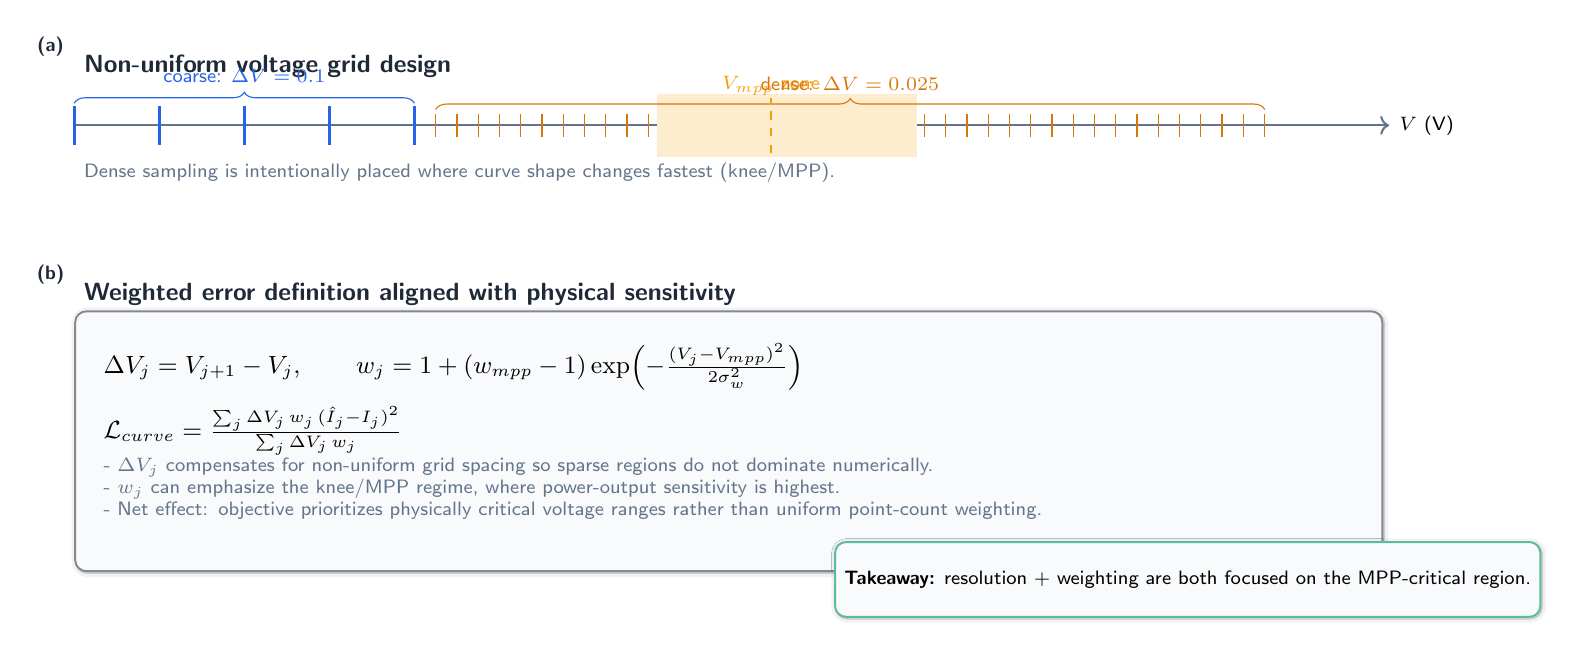
\begin{tikzpicture}[every node/.style={font=\sffamily\scriptsize}]

\node[figlabel] at (-0.3,2.8) {(a)};
\node[figtitle, anchor=west] at (0,2.55) {Non-uniform voltage grid design};

\draw[->, line width=0.75pt, draw=figMuted] (0,1.8) -- (16.7,1.8) node[right] {$V$ (V)};
% coarse region 0..0.4
\foreach \v in {0.0,0.1,0.2,0.3,0.4} {
  \pgfmathsetmacro{\x}{\v*10.8}
  \draw[draw=figBlue, line width=1.0pt] (\x,1.55) -- (\x,2.05);
}
% dense region 0.425..1.4
\foreach \i in {0,...,39} {
  \pgfmathsetmacro{\v}{0.425 + 0.025*\i}
  \pgfmathsetmacro{\x}{\v*10.8}
  \draw[draw=figAmber, line width=0.45pt] (\x,1.65) -- (\x,1.95);
}
\fill[figMpp!20] (7.4,1.4) rectangle (10.7,2.2);
\draw[draw=figMpp, line width=0.9pt, dashed] (8.85,1.45) -- (8.85,2.15);
\node[text=figMpp] at (8.85,2.3) {$V_{mpp}$ zone};
\draw[decorate, decoration={brace, amplitude=4pt}, draw=figBlue] (0,2.08) -- (4.32,2.08);
\node[text=figBlue, anchor=south] at (2.16,2.22) {coarse: $\Delta V=0.1$};
\draw[decorate, decoration={brace, amplitude=4pt}, draw=figAmber] (4.59,2.0) -- (15.12,2.0);
\node[text=figAmber, anchor=south] at (9.85,2.12) {dense: $\Delta V=0.025$};
\node[fignote, anchor=west] at (0,1.2)
{Dense sampling is intentionally placed where curve shape changes fastest (knee/MPP).};

\node[figlabel] at (-0.3,-0.1) {(b)};
\node[figtitle, anchor=west] at (0,-0.35) {Weighted error definition aligned with physical sensitivity};

\node[figbox, minimum width=16.6cm, minimum height=3.3cm, anchor=north west] (eq) at (0,-0.55) {};
\node[anchor=north west, font=\sffamily\small] at (0.25,-0.85)
{$\Delta V_j = V_{j+1}-V_j,\qquad
w_j = 1 + (w_{mpp}-1)\exp\!\left(-\frac{(V_j-V_{mpp})^2}{2\sigma_w^2}\right)$};
\node[anchor=north west, font=\sffamily\small] at (0.25,-1.65)
{$\mathcal{L}_{curve}=\frac{\sum_j \Delta V_j\,w_j\,(\hat I_j-I_j)^2}{\sum_j \Delta V_j\,w_j}$};
\node[fignote, anchor=north west, text width=16.0cm] at (0.25,-2.3)
{- $\Delta V_j$ compensates for non-uniform grid spacing so sparse regions do not dominate numerically.\\
- $w_j$ can emphasize the knee/MPP regime, where power-output sensitivity is highest.\\
- Net effect: objective prioritizes physically critical voltage ranges rather than uniform point-count weighting.};

\node[figbox, minimum width=6.8cm, minimum height=0.95cm, draw=figGreen!65, anchor=north west] at (9.65,-3.48)
{\textbf{Takeaway:} resolution + weighting are both focused on the MPP-critical region.};

\end{tikzpicture}
\end{document}
